%%%%%%%%%%%%%%%%%%%%%%%%%%%%%%%%%%%%%%%%%
% Beamer Presentation
% LaTeX Template
% Version 1.0 (10/11/12)
%
% This template has been downloaded from:
% http://www.LaTeXTemplates.com
%
% License:
% CC BY-NC-SA 3.0 (http://creativecommons.org/licenses/by-nc-sa/3.0/)
%
%%%%%%%%%%%%%%%%%%%%%%%%%%%%%%%%%%%%%%%%%

%----------------------------------------------------------------------------------------
%	PACKAGES AND THEMES
%----------------------------------------------------------------------------------------

\documentclass{beamer}

\mode<presentation> {
	
	% The Beamer class comes with a number of default slide themes
	% which change the colors and layouts of slides. Below this is a list
	% of all the themes, uncomment each in turn to see what they look like.
	
	%\usetheme{default}
	%\usetheme{AnnArbor}
	%\usetheme{Antibes}
	%\usetheme{Bergen}
	%\usetheme{Berkeley}
	%\usetheme{Berlin}
	%\usetheme{Boadilla}
	%\usetheme{CambridgeUS}
	%\usetheme{Copenhagen}
	%\usetheme{Darmstadt}
	%\usetheme{Dresden}
	%\usetheme{Frankfurt}
	%\usetheme{Goettingen}
	%\usetheme{Hannover}
	%\usetheme{Ilmenau}
	%\usetheme{JuanLesPins}
	%\usetheme{Luebeck}
	\usetheme{Madrid}
	%\usetheme{Malmoe}
	%\usetheme{Marburg}
	%\usetheme{Montpellier}
	%\usetheme{PaloAlto}
	%\usetheme{Pittsburgh}
	%\usetheme{Rochester}
	%\usetheme{Singapore}
	%\usetheme{Szeged}
	%\usetheme{Warsaw}
	
	% As well as themes, the Beamer class has a number of color themes
	% for any slide theme. Uncomment each of these in turn to see how it
	% changes the colors of your current slide theme.
	
	%\usecolortheme{albatross}
	%\usecolortheme{beaver}
	%\usecolortheme{beetle}
	%\usecolortheme{crane}
	%\usecolortheme{dolphin}
	%\usecolortheme{dove}
	%\usecolortheme{fly}
	%\usecolortheme{lily}
	%\usecolortheme{orchid}
	%\usecolortheme{rose}
	%\usecolortheme{seagull}
	%\usecolortheme{seahorse}
	%\usecolortheme{whale}
	%\usecolortheme{wolverine}
	
	%\setbeamertemplate{footline} % To remove the footer line in all slides uncomment this line
	%\setbeamertemplate{footline}[page number] % To replace the footer line in all slides with a simple slide count uncomment this line
	
	%\setbeamertemplate{navigation symbols}{} % To remove the navigation symbols from the bottom of all slides uncomment this line
}

\usepackage{graphicx} % Allows including images
\usepackage{booktabs} % Allows the use of \toprule, \midrule and \bottomrule in tables
\usepackage{epigraph}

%----------------------------------------------------------------------------------------
%	TITLE PAGE
%----------------------------------------------------------------------------------------

\title[Intro to probability]{An introduction to probability} % The short title appears at the bottom of every slide, the full title is only on the title page

\author{Ben Lambert} % Your name
\institute[Univ. of Oxford] % Your institution as it will appear on the bottom of every slide, may be shorthand to save space
{
	University of Oxford \\ % Your institution for the title page
	\medskip
	\textit{ben.c.lambert@gmail.com} % Your email address
}
\date{\today} % Date, can be changed to a custom date

\begin{document}
	
	\begin{frame}
		\titlepage % Print the title page as the first slide
	\end{frame}

	\begin{frame}
		\frametitle{Who am I?}
		
		\begin{itemize}
			\item Statistician working mainly in epidemiology.
			\item Claim to probability fame: born in the same town where Thomas Bayes lived (Tunbridge Wells, UK).
		\end{itemize}
		
		\begin{figure}[ht]
			\centerline{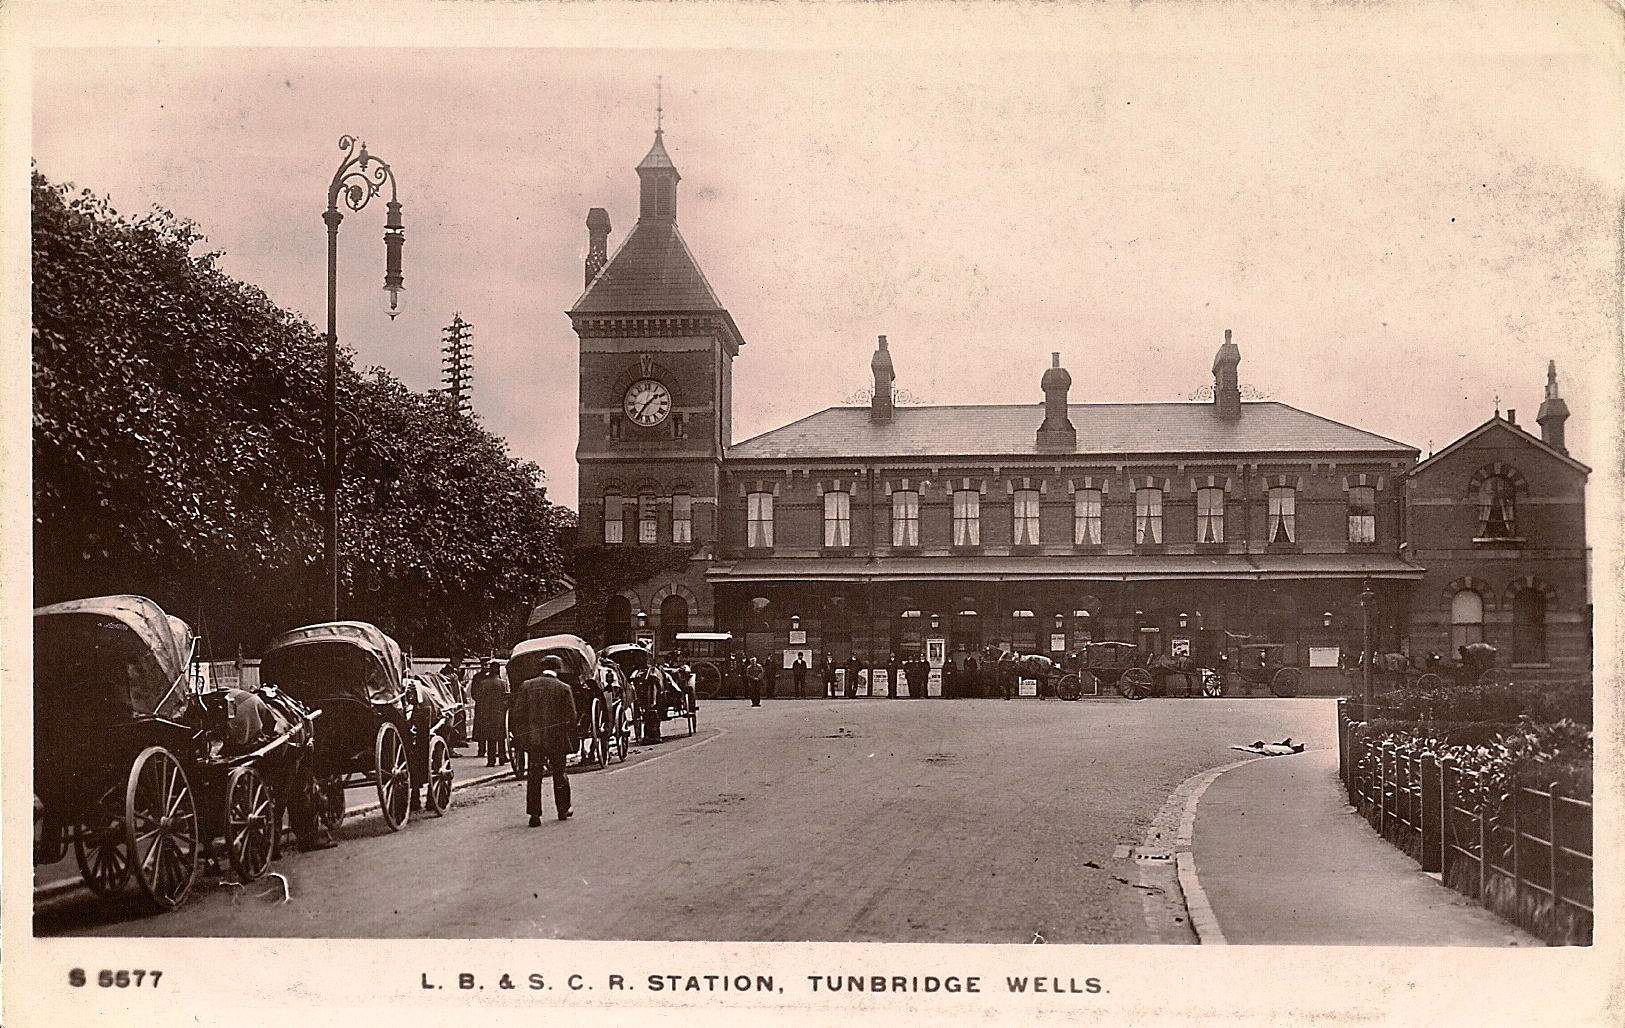
\includegraphics[width=0.6\textwidth]{./figures/tunbridgeWells.jpg}}
		\end{figure}
		
	\end{frame}

	\begin{frame}
		\frametitle{Course outline}
		
		\begin{itemize}
			\item 9am-10.30am: follow along lecture and problems
			\item 10.30am-10.45am: refreshments break
			\item 10.45am-midday: follow along lecture and problems
		\end{itemize}
		
	\end{frame}

	\begin{frame}
		\frametitle{Resources}
		
		\begin{itemize}
			\item Introduction to probability, Blitzstein and Hwang. Open source book available here: \url{https://projects.iq.harvard.edu/stat110/home}
			\item Seeing theory, Kunin et al. A beautiful online resource that has lots of creative ways to think about probability. \url{https://seeing-theory.brown.edu/}
		\end{itemize}
		
	\end{frame}

	\begin{frame}
		\frametitle{Outline}
		\tableofcontents
	\end{frame}

	\section{What is probability and why do we need it?}
	\frame{\tableofcontents[currentsection]}
	
	\begin{frame}
		\frametitle{What is probability?}
		\epigraph{Mathematics is the logic of certainty; probability [theory] is the [mathematical] logic of uncertainty}{Bitzstein and Hwang, 2019}
		
	\end{frame}

	\begin{frame}
		\frametitle{Why do we need probability theory?}
		
		Life and science are full of unknown things. We say these things are \textit{uncertain}.
		
		Faced with these, we can give up; \textit{Probability theory} gives us a way to make assumptions about uncertain phenomena which allows us to make progress with understanding without having to know everything.
		
		\epigraph{There are known knowns. These are things we know that we know. There are known unknowns. That is to say, there are things that we know we don't know. But there are also unknown unknowns. There are things we don't know we don't know.}{Donald Rumsfeld, 2002}
		
	\end{frame}
	
	\begin{frame}
		\frametitle{Who uses probability?}
		It is used in:
		
		\begin{itemize}
			\item Statistics: probability is the foundational language of it
			\item Biology: e.g. inheritance of genes
			\item Meteorology: e.g. weather forecasts are generated using probabilities
			\item Epidemiology: e.g. analysing randomised clinical trials and fitting models to epidemiological data
			\item Physics: our current best explanation of the universe at small scales (quantum theory) is based on probability
		\end{itemize}
		
		
	\end{frame}

	\begin{frame}
		\frametitle{The difficulties of probability}
		
		If we rely on our intuitions, it is easy to go awry with probability.
		
		\vspace{0.5cm}
		
		 So, we need careful mathematical analysis.
		 
		 \vspace{0.5cm}
		
		Fortunately, \textit{simulation} using R / Python / etc. can also really help us to understand.
		
	\end{frame}

	\section{Probability and counting}
	\frame{\tableofcontents[currentsection]}
	
	\begin{frame}
		\frametitle{Blitzstein and Hwang's Pebble World}
		
		As an example, consider reaching into a bag to pull out one of nine pebbles: we call this \textit{pebble world}.
		
		\begin{figure}[ht]
			\centerline{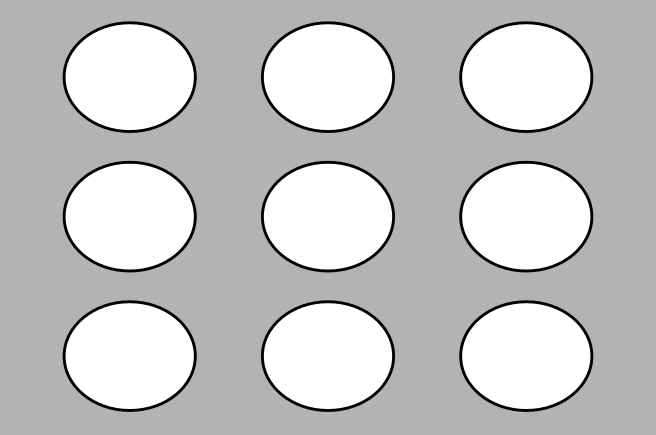
\includegraphics[width=0.6\textwidth]{./figures/pebble_world_base.png}}
		\end{figure}
		
	\end{frame}


	\begin{frame}
		\frametitle{Outcomes}
		
		An \textit{outcome} is a possible result of some activity. Here pulling one particular pebble out of the bag would be an outcome.
		
		\begin{figure}[ht]
			\centerline{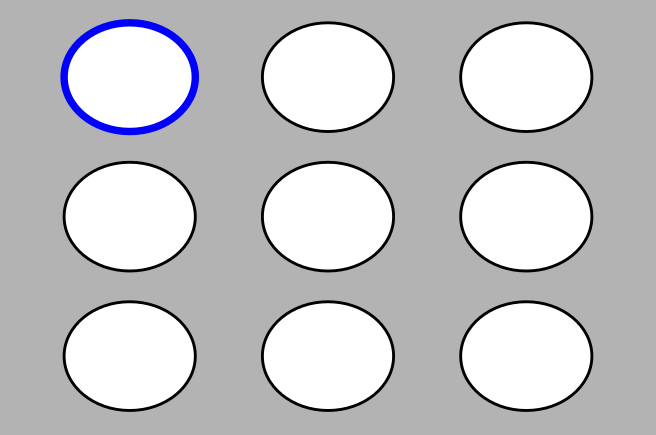
\includegraphics[width=0.6\textwidth]{./figures/pebble_world_single.png}}
		\end{figure}
		
	\end{frame}

	\begin{frame}
		\frametitle{Sample spaces}
		
		The \textit{sample space}, $S$, is the \textit{set} of all possible outcomes of an experiment. Here, it is the set of all pebbles.
		
		\begin{figure}[ht]
			\centerline{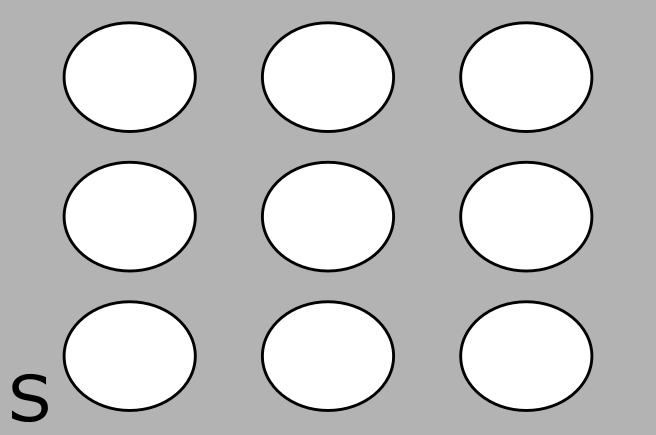
\includegraphics[width=0.6\textwidth]{./figures/pebble_world_sample_space.png}}
		\end{figure}
		
	\end{frame}

	\begin{frame}
		\frametitle{Events}
		
		An \textit{event} is a \textit{set} of possible outcomes. For example, below event $A$ corresponds to selecting one of five pebbles; event $B$ to selecting one of two.
		
		As we can see, two or more events can happen at once.
		
		\begin{figure}[ht]
			\centerline{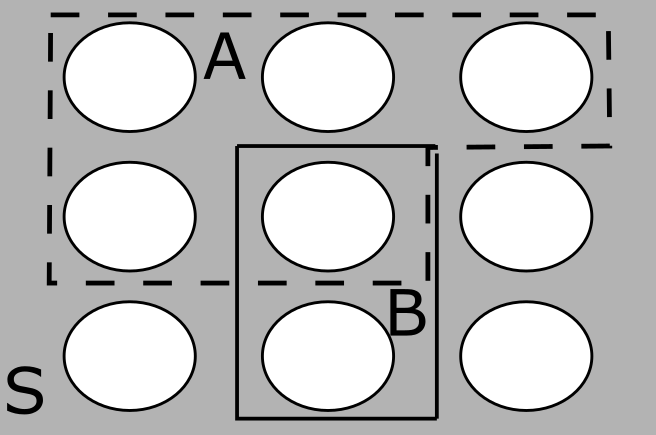
\includegraphics[width=0.6\textwidth]{./figures/pebble_world.png}}
		\end{figure}
		
	\end{frame}


	\begin{frame}
		\frametitle{Probabilities of events}
		
		What do we mean by the probability of $A$ occurring? We write this as: $\mathbb{P}(A)$.
		
		\begin{figure}[ht]
			\centerline{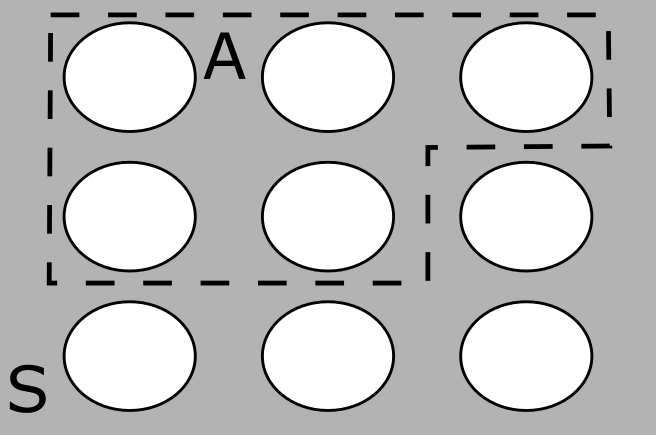
\includegraphics[width=0.6\textwidth]{./figures/pebble_world_proba.png}}
		\end{figure}
		
	\end{frame}

	\begin{frame}
		\frametitle{Probabilities from counting}
		
		If all pebbles equally likely to be drawn:
		
		 \begin{equation}
		 	\mathbb{P}(A) = \frac{\text{number of pebbles in } A}{\text{number of pebbles in } S} = \frac{5}{9}
		 \end{equation}
	 
	 \begin{figure}[ht]
	 	\centerline{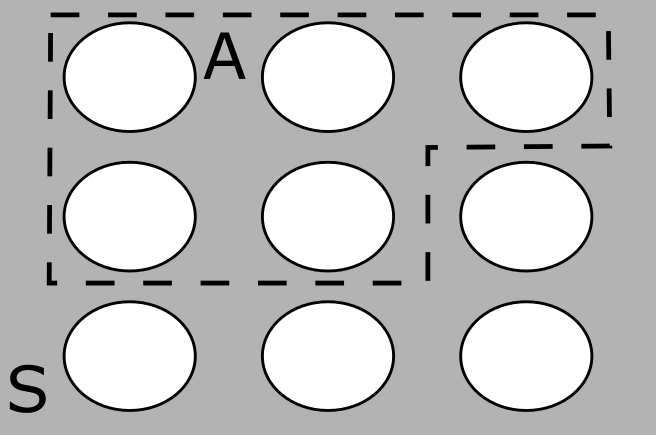
\includegraphics[width=0.6\textwidth]{./figures/pebble_world_proba.png}}
	 \end{figure}
		
	\end{frame}

	\begin{frame}
		\frametitle{Probability of an event in $S$}
		
		Consider the probability that some event in $S$ occurs:
		
		\begin{equation}
			\mathbb{P}(S) = \frac{\text{number of pebbles in } S}{\text{number of pebbles in } S} = \frac{9}{9} = 1
		\end{equation}
		
		\begin{figure}[ht]
			\centerline{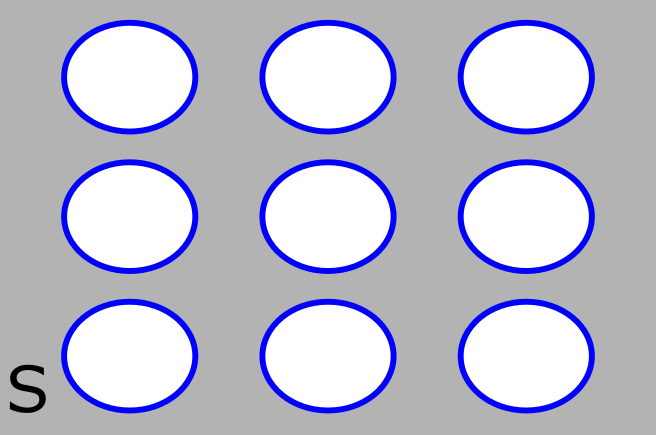
\includegraphics[width=0.6\textwidth]{./figures/pebble_world_probs.png}}
		\end{figure}
		
	\end{frame}

	\begin{frame}
		What about the probability that no event in $S$ occurs?
		
		\begin{equation}
			\mathbb{P}(\text{not }S) = \frac{0}{9} = 0
		\end{equation}
		
		\begin{figure}[ht]
			\centerline{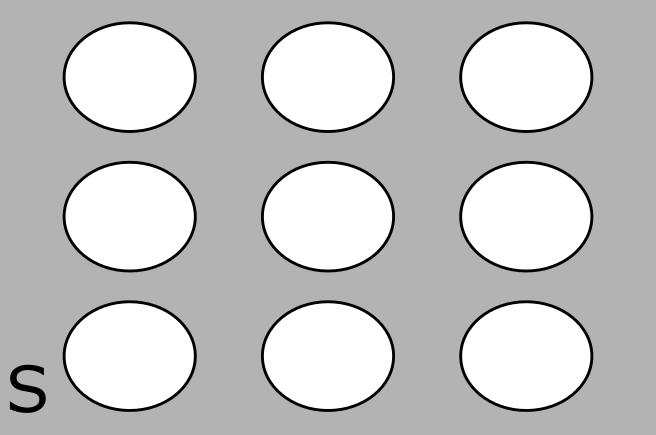
\includegraphics[width=0.6\textwidth]{./figures/pebble_world_probnots.png}}
		\end{figure}
		
	\end{frame}

	\begin{frame}
		\frametitle{Defining a probability}
		
		A probability of an event must be bounded between 0 and 1\footnote{Note: ``impossible'' isn't 100\% accurate here but you can start out by thinking of probabilities this way.}.
		
		\begin{figure}[ht]
			\centerline{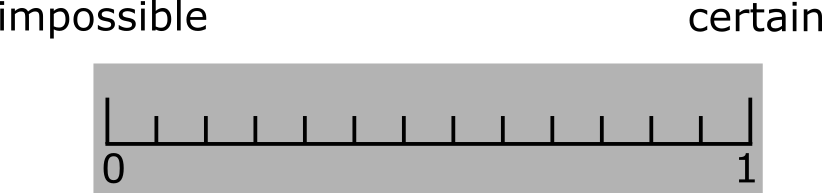
\includegraphics[width=0.8\textwidth]{./figures/probability.png}}
		\end{figure}
		
	\end{frame}

		\begin{frame}
		\frametitle{An event not occurring}
		We can also determine the probability that $A$ does not occur:
		
		\begin{equation}
			\mathbb{P}(\text{not } A) = \frac{\text{number of pebbles not in } A}{\text{number of pebbles in } S} = \frac{4}{9}
		\end{equation}
		
		\begin{figure}[ht]
			\centerline{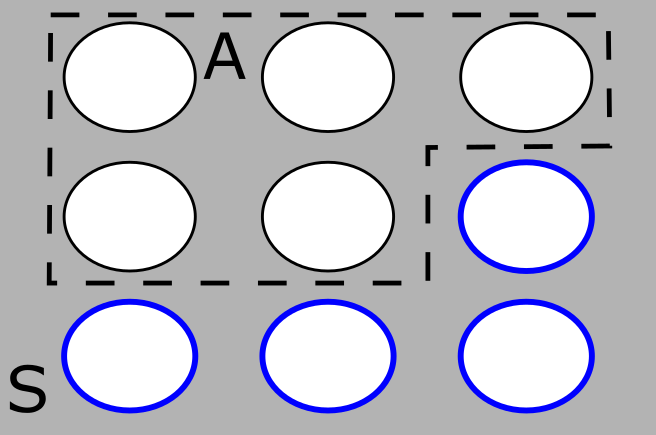
\includegraphics[width=0.6\textwidth]{./figures/pebble_world_probnota.png}}
		\end{figure}
		
	\end{frame}

	\begin{frame}
		\frametitle{Question}
		
		\Large Can anyone think of an alternative way of determining the probability that $A$ does not occur?
		
	\end{frame}

	\begin{frame}
		\frametitle{Question}
		
		\Large Can anyone think of an alternative way of determining the probability that $A$ does not occur?
		
		\begin{equation}
			\mathbb{P}(\text{not } A) = \mathbb{P}(S) - \mathbb{P}(A) = 1 - \mathbb{P}(A) = 1 - \frac{5}{9}
		\end{equation}
		
	\end{frame}

	\begin{frame}
		\frametitle{Combinations of events: intersection}
		
		We can determine the probability of $A$ \textit{and} $B$ occurring by determining the overlap between these two events:
		
		\begin{equation}
			\mathbb{P}(A \cap  B) = \mathbb{P}(A, B) = \frac{\text{number of pebbles in both } A \text{ and } B}{\text{number of pebbles in } S} = \frac{1}{9}
		\end{equation}
		
		\begin{figure}[ht]
			\centerline{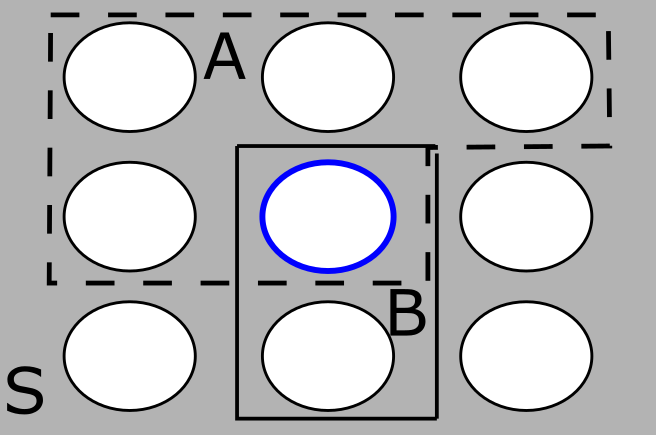
\includegraphics[width=0.6\textwidth]{./figures/pebble_world_and.png}}
		\end{figure}
		
	\end{frame}

	\begin{frame}
		\frametitle{Combinations of events: union}
		
		We can determine the probability of $A$ \textit{and/or} $B$ occurring by:
		
		\begin{equation}
			\mathbb{P}(A \cup B) = \frac{\text{number of pebbles in either } A \text{ or } B \text{ or both}}{\text{number of pebbles in } S} = \frac{6}{9}
		\end{equation}
	
	\begin{figure}[ht]
		\centerline{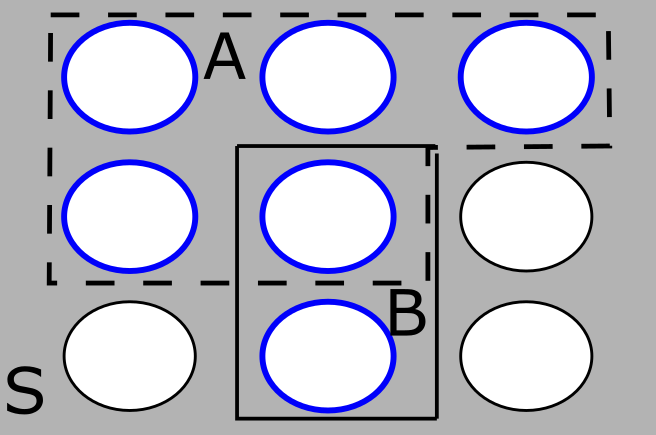
\includegraphics[width=0.6\textwidth]{./figures/pebble_world_or.png}}
	\end{figure}
		
	\end{frame}

	\begin{frame}
		\frametitle{Question}
		
		\Large Can anyone think of an alternative way of determining the probability of the union of $A$ and $B$?
		
	\end{frame}

	\begin{frame}
		\frametitle{Question}
		
		\Large Can anyone think of an alternative way of determining the probability of the union of $A$ and $B$?
		
		\begin{align}
			\mathbb{P}(A \cup B) &= \mathbb{P}(A) + \mathbb{P}(B) - \mathbb{P}(A \cap B)\\
			&= \frac{5}{9} + \frac{2}{9} - \frac{1}{9} = \frac{6}{9}
		\end{align}
		
		
	\end{frame}
	
	
	\begin{frame}
		\frametitle{}
		\Large Questions?
	\end{frame}
	
	
	\begin{frame}
		\frametitle{Problems}
		
		\begin{figure}[ht]
			\centerline{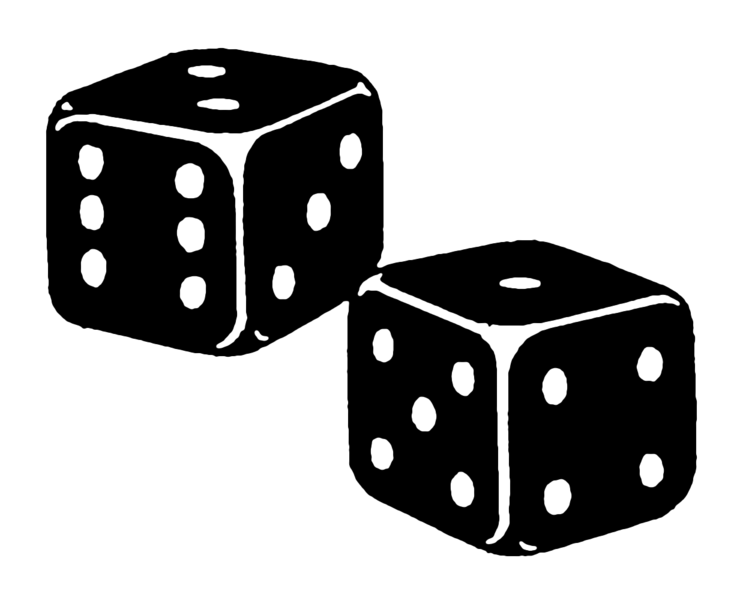
\includegraphics[width=0.3\textwidth]{./figures/dice.png}}
		\end{figure}
	
	Consider a six-sided die with numbers 1-6 on each face that is thrown once.
		
		\begin{enumerate}
			\item What's the probability that a six is thrown?
			\item What's the probability that an even number is thrown?
			\item What's the probability that either an even number or one is thrown?
		\end{enumerate}
		
	\end{frame}


	\section{Probability distributions}


	\section{Joint distributions}
	\frame{\tableofcontents[currentsection]}

	\section{Marginal and conditional probability}
	\frame{\tableofcontents[currentsection]}
	
	\section{Bayes' rule}
	\frame{\tableofcontents[currentsection]}
	
	Use breast cancer example.
	
	\section{Continuous probability distributions}
	\frame{\tableofcontents[currentsection]}
	
\end{document} 